%% \section{Results and Discussion}
%% \label{sec:results}

%% In this section we present the main findings of our research. We first present the results of each study (Section~\ref{sec:survey-resuts}, Sections~\ref{sec:msr-results}, and Section~\ref{sec:interview-results}). After that, in Section~\ref{sec:discussion} we consolidate our findings and present some implications of our study. 

\section{Results of the Survey}
\label{sec:survey-resuts} 

Our first study investigates the impact of atoms of confusion while developers try to understand JavaScript code.
We estimate this impact considering two perspectives: \emph{misunderstanding rate} (number of wrong answers)
and \emph{cognitive effort} (time necessary to provide a correct answer). We receive full answers to our survey
from 140 participants. Figure~\ref{fig:degree} and Figure~\ref{fig:xp} show the distributions of the subjects,
according to their education level and years of programming experience, respectively.

\begin{figure}[htb]
      \centering
      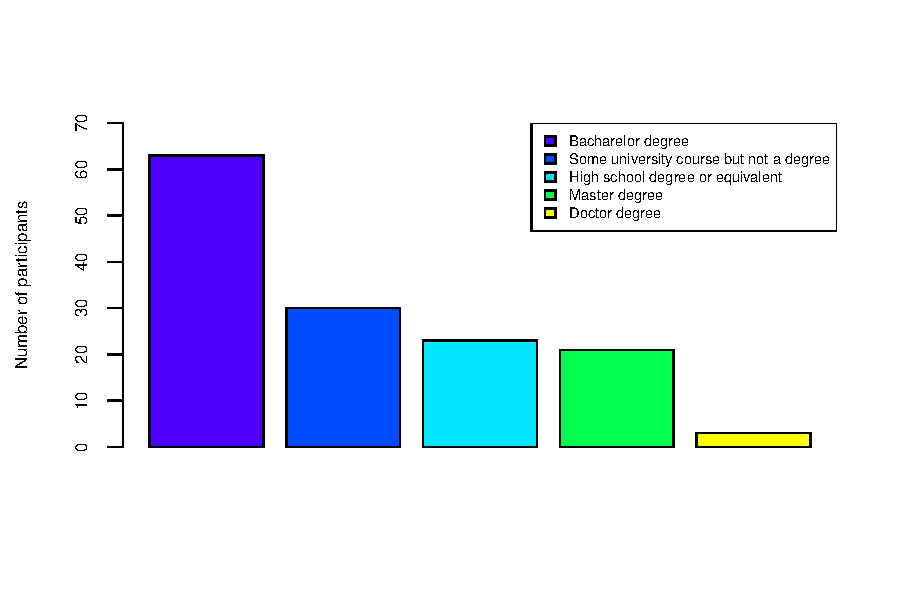
\includegraphics[width=\columnwidth]{images/dem-education-1.pdf}
      \caption{Participants' Education Level}\label{fig:degree}
  \end{figure}
  
  \begin{figure}[htb]
      \centering
      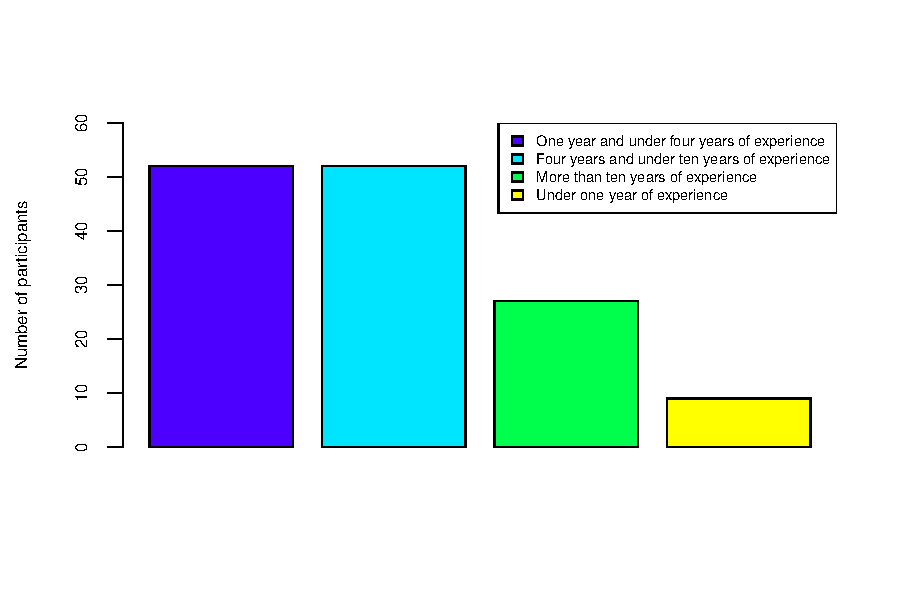
\includegraphics[width=\columnwidth]{images/dem-experience-1.pdf}
      \caption{Participants' Experience} \label{fig:xp}
  \end{figure}

Figure~\ref{fig:xp} shows that more than a half of the participants hold either a BS degree or had taken some university course, meaning the participants have had some level of formal education on programming. No subject reported to have never attended university. Our audience comprises skillful developers, and 93\% of the respondents have more than one year of experience with programming (see Figure~\ref{fig:xp}). Actually, 56\% of the participants have either between four and ten years of experience (37\%) or more than ten years of experience (19\%). Other 37\% of the respondents have between one and four years of experience. In this way, we characterize the effect of atoms of confusion in JavaScript code taking into account the perceptions of both novice and experience developers. 

\subsection{Misunderstanding Analysis}

\subsubsection*{Exploratory Data Analysis}

Each participant in this study evaluated {\color{red}10} code snippets, from which 5 were in their confusing versions, whilst the other 5 contained cleaned versions of the code snippets (i.e., without the confusing constructs and idioms). The participants should provide the expected outcomes of the code snippets. We collected information about \emph{correctness} (whether the participant correctly predicted the program's output) and \emph{cognitive workload} (the time taken to answer the question). Our final dataset consists of 70 complete Latin Squares.


Regarding \emph{correctness}, Table~\ref{results_correctness} and Figure~\ref{fig:boxplotcorrectness} summarize the results of the survey. Accordingly, the version of seven code snippets without atoms of confusion present at least a 15\% improvement in answer correctness. In particular, \emph{Comma Operator} atom presents the highest impact on misunderstanding. 
Curiously, frequently used constructs and idioms, such as \emph{Post Increment} and \emph{Omitted Curly Braces} (see Section~\ref{sec:msr-results}), also introduce high degrees of confusion.

Moreover, as the boxplot in Figure \ref{fig:boxplotcorrectness} shows, there is a considerable decrease in the average number of incorrect answers when observing the cleaned version of the code snippets. Also, the sample of answers where there was no atoms had almost no dispersion, which is a sign that the non-confusing code is easier to evaluate correctly.

% \begin{table}[htbp]
% \caption{Difference in answer correctness between confusing and non-confusing pairs}
% \begin{center}
% \begin{small}
% \begin{tabularx}
% {{\linewidth}}{l p{1.5cm} p{1.1cm} p{1.1cm} p{1.2cm} }
% \textbf{Atom} & \textbf{\%Correct} & \textbf{\%Correct} \\
% &  \multicolumn{1}{l}{With AOC} \multicolumn{2}{l}{Without AOC}  & \Delta (\%)    \\
%  \hline
% Comma Operator & 40 & 93 & +132\%                 \\     
% Automatic Semicolon  Insertion & 46 & 97 & +110\% \\
% Post Increment & 69 & 91 & +31\%         \\
% Omitted Curly Braces & 67 & 83 & +23\%   \\ 
% Assignment as Value & 80 & 97 & +21\%    \\
% Implicit Predicate & 83 & 97 & +16\%     \\
% Logic as Control Flow & 59 & 68 & +15\%  \\
% Ternary Operator & 86 & 94 & +9\%        \\
% Pre-Increment & 71 & 76 & +7\%           \\
% Arithmetic as Logic & 91 & 90 & -1\%    \\
% \end{tabularx}
% \end{small}
% \end{center}
% \label{results_correctness}
% \end{table}

\begin{table*}[htbp]
\caption{Total number of correct answers.}
\label{tab:difference-correctness}
\centering{
\begin{tabular}{lccc|c} \toprule
 % & \multicolumn{2}{c}{Total Number of Correct Answers} & \\ [0.1cm]
  Atom & Confuse Code & Clean Code & $\Delta$(\%) & Effect Size (Odds Ratio) \\ \midrule
  Comma Operator &  28 &  65 & +132 & 19.02 \\ 
  {\color{red}Automatic Semicolon Insertion} &  32 &  68 & +112 & 39.32 \\ 
  Post Increment &  48 &  64 & +33 & 4.83 \\ 
  Ommitted Curly Braces &  47 &  58 &  +23 & 2.35 \\
  Assignment as Value &  56 &  68 &  +21 & 8.38 \\ 
  Implict Predicate &  58 &  68 &  +17 & 6.94 \\ 
  Logic as Control Flow &  41 &  48 &  +17 & 1.53 \\ 
  Ternary Operator &  60 &  66 &  +10 & 2.73 \\ 
  Pre Increment &  50 &  53 &  +6 & 1.24 \\ 
  Arithmetic as Logic &  64 &  63 &  -2 & 0.84 \\ \bottomrule 
\end{tabular}
}
\end{table*}

 %% Comma Operator          & 40 & 93  & +132 \\
 %% Post Increment          & 69 & 91  & + 31  \\
 %% Omitted Curly Braces    & 67 & 83  & +23 \\
 %% Assignment as Value     & 80 & 97  & +21 \\
 %% Implicit Predicate      & 83 & 97  & +16 \\
 %% Logic as Control Flow   & 59 & 68  & +15 \\
 %% Ternary Operator        & 86 & 94  & +9  \\
 %% Pre-Increment           & 71 & 76  & +7  \\
 %% Arithmetic as Logic     & 91 & 90  & +1  \\ \bottomrule


\begin{figure}[htb!]
\noindent
 \centering
 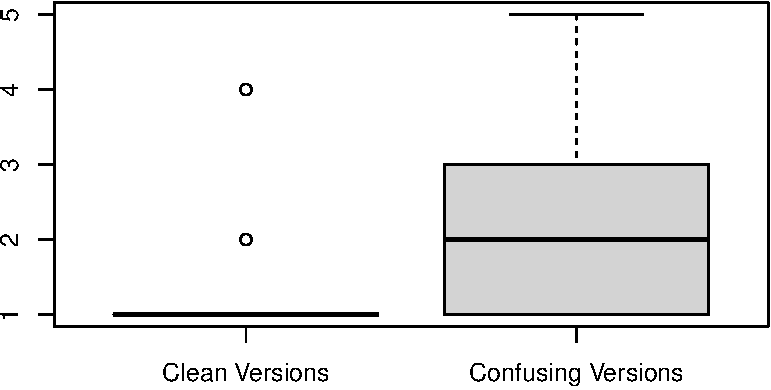
\includegraphics[width=\columnwidth]{images/wrong-answers-plot-1.pdf}
 \caption{Number of wrong answers of each subject}
 \label{fig:boxplotcorrectness}
 \end{figure}

\rb{verificar a consistencia nas questoes de pesquisa mais especificas}

\subsubsection*{Hypothesis Testing and Effect Size}

We first use the \emph{Pearson's Chi-squared test}
to investigate if there is a statistically significant difference
in the frequency of correct and incorrect answers---due to the versions
of the code snippets (confuse and clean code). The result shows that the confusing version of the code snippets impacts code understanding (p-value $< 0.05$). We also use the \emph{Binomial Generalized Logistic Regression} analysis to investigate if either participant
\emph{education} or participant \emph{experience} impact on correctness. Although the results suggest that experience impact correctness, the education level does not. We then replicate the \emph{Pearson's Chi-squared test} for each experience group (see Figure~\ref{fig:xp}) and found that the statistic difference is less significant for those developers with more than ten years of experience.
Finally, we measure the effect size of the clean version of the code snippets into the answers' correctness, using the \emph{Odds Ratio} (OR)
method (see Table~\ref{tab:difference-correctness}). We found a negligible effect size for the atom candidates Arithmetic as Logic, Logic as Control Flow, and Pre Increment. Nonetheless, for the remaining candidates, the effect size is considerable. For instance, the Comma Operators leads to an \emph{Odds Ratio} of
\num{19.02}, meaning that the the odds of a correct answer are \num{19.02} times
higher when interpreting the clean version of a code---in comparison with the corresponding, confuse version of the code snippet.


%% Regarding the first question we 
%% address in the survey (\emph{Do code snippets that contain atoms of confusion produce a higher error rate than snippets where the atom is removed?}), we found evidence that the atoms of confusion lead programmers to misunderstand JavaScript code. We also realized that just one atom whose correction has a non-significant improvement in the percentage of correct answers---we found an improvement of at least 15\% in the correct answers when removing the confusing code for seven atoms (out of ten atoms we consider in the survey). 

\subsection{Cognitive Workload Analysis}

\subsubsection*{Exploratory Data Analysis}
Table \ref{tab:difference-time-taken} shows the average time necessary for the participants give a correct answer about the expected outcomes of a code snippet, considering both confuse and clean versions. Eight atom candidates require an increasing cognitive workload. For these eight atom candidates, developers take at least 5.90\% less time on average to find a correct answer---when considering the clean version of a code snippet. In the extreme case (atom candidate Comma Operator), the participants take 76.23\% less
time on average to find the correct answer for the clean version of the code snippets. 
Not all atom candidates, though, take less time to predict the answer. In fact, for the Arithmetic as Logic and the Pre-Increment atoms, there was an increase
of 29.06\% and 38.19\% in the average time taken to give a correct answwer---wherein the clean code versions.

\begin{table*}[htbp]
\caption{Time in seconds to submit a {\color{red}correct} answer}
\label{tab:difference-time-taken}
\centering{
\begin{tabular}{lccc|cc} \toprule
Atom & Confuse Code & Clean Code & $\Delta$(\%) & Mann-Whitney test & Cliff's Delta \\ \midrule 
Comma Operator & 87.67 & 20.84 & -76.23 &  \colorbox{lightgray}{$<$ 0.01} & -0.53 \\ 
Logic as Control Flow & 108.94 & 51.07 & -53.12 &  \colorbox{lightgray}{$<$ 0.01} & -0.39 \\ 
{\color{red}Automatic Semicolon Insertion} & 46.08 & 22.04 & -52.17 & 0.09 & -0.16 \\ 
Ommitted Curly Braces & 48.85 & 30.00 & -38.58 & 0.92 & -0.01 \\ 
Implict Predicate & 36.24 & 24.01 & -33.75 & \colorbox{lightgray}{$<$ 0.01} & -0.29 \\ 
Post Increment & 28.70 & 25.67 & -10.56 & 0.12 & 0.15 \\ 
Assignment as Value & 52.47 & 48.95 & -6.71 & 0.82 & 0.02 \\ 
Ternary Operator & 41.80 & 39.34 & -5.90 & 0.24 & -0.12 \\ 
Arithmetic as Logic & 28.82 & 37.20 & +29.06 & \colorbox{lightgray}{0.01} & 0.23 \\ 
Pre Increment & 30.71 & 42.45 & +38.19 & \colorbox{lightgray}{$<$ 0.01} & 0.27 \\ 
         \bottomrule
    \end{tabular}}
\end{table*}


\subsubsection*{Hypotheis Testing}
We use the non-parametric \emph{Mann-Whitney test} to
investigates the null hypothesis that developers 
spend the same ammount of time to correctly
predict the outcome of a code snippet, regardless
of evaluating the confuse or the clean version
of the code. Table~\ref{tab:difference-time-taken}
shows the results, which suggest that we
should refute the null hypothes for
five atom candidates (Comma Operator, Logic
as Control Flow, Implicit Predicate, Arithmetic
as Logic, and Pre Increment). For the first three,
the analysis suggest that the participants
need more time to predict the outcome of
the code snippet in the confuse code version. Interesting,
for the atom candidates Arithmetic as Logic and
Pre Increment, the participants take less time
to predict the outcome of the code snippets in
the confuse version.
We also computed the effect size using the Cliff's Delta method.
We found a large effect for the Comma Operator atom
candidate; and a moderate effect for the atom candidates
Logic as Control Flow, Implicit Predicate, Arithmetic
as Logic, and Pre Increment. 

\rb{Acho que dever\'{i}mos justificar o uso do Cliff's Delta aqui e o Odds Ratio na
  se\c c\~{a}o anterior.}

\subsection{Discussion}

\rb{Acho que podemos incluir uma discuss\~{a}o ao
  t\'{e}ermino de cada uma das se\c c\~{o}es com
  resultados. Ou separamos em uma \'{u}nica
se\c c\~{a}o de discuss\~{a}o?}




%%  Comma Operator        & 60 & 21  & -65  \\
%% Logic as Control Flow & 85 & 49  & -42  \\
%% Implicit Predicate    & 33 & 24  & -27  \\
%% Omitted Curly Braces  & 43 & 31  & -27  \\
%% Assignment as Value   & 53 & 49  & -7   \\
%% Ternary Operator      & 42 & 42  & 0    \\
%% Post Increment        & 27 & 27  & 0    \\
%% Arithmetic as Logic   & 29 & 36  & +24  \\
%% Pre-Increment         & 34 & 49  & +44  \\


\
% \rb{acho que podemos melhorar a apresenta\c c\~{a}o dessas tabelas, talvez usando booktabs.}


\section{Results of the Interview Study}
\label{sec:interview-results}

\rb{acho que essa separa\c c\~{a}o em dois rounds est\'{a}
  gerando uma complexidade desnecess\'{a}ria. vou tentar
  remover isso}.

In this section we present the results of the 
interviews with the practitioners who agreed to participate
in the study. A total of 15 practitioners
took part of the interviews.
We collected information regarding programming
experience, familiarity with JavaScript, and their opinion
about the {\color{red}nine} atom candidates---by
(a) presenting them pairs of code snippets whose behavior were identical
and then (b) asking them to compare the code snippets readability.

%% In the second round of interviews, ten of the fifteen developers
%% who participated in the first round were shown another 8 atom candidates to atom of confusion whose frequency we observed during the repository mining phase. The same procedure of showing code that behaves exactly the same and surveying for how easy to understand each snippet was applied in this phase. 

Supporting the results of the survey, Tables~\ref{tab:interview-results1}
and~\ref{tab:interview-results2} show that for twelve out of the
seventeen scenarios surveyed, the respondents prefer the version of the
code without the atom of confusion, and in no case the \emph{neutral}
ratio was higher than the option for the version without atoms of confusion.
%% An example entry is contained in Appendix~\ref{}. 
%% For a full listing of the code snippets, visit the paper repository. 

\subsubsection*{Participants views of the atoms} Interesting,
only for the \emph{ternary operator} scenario the participants
prefer the version of the code with the atom of confusion,
instead of the more cleaner version without the atom of confusion.
Even in this case, some participants who opted for
the \emph{left-hand-side} (with the atom of confusion) version
still believed that the \emph{right-hand-side} (without the atom of
confusion) version was more readable (see Figure~\ref{code:ternary}). 
The following quotes were extracted from the transcripts with
three inteviwes:

\begin{figure*}

\noindent\begin{minipage}{.45\textwidth}
\begin{lstlisting}[language=JavaScript, caption=\emph{Left-hand side} (using the \emph{Ternary Operator} atom)]
let config = {size: 3, isActive: false};
const_config = config.isActive === true 
             ? config 
             : {size: 10};
console.log(_config.size);
\end{lstlisting}
\end{minipage}\hfill
\begin{minipage}{.45\textwidth}
\begin{lstlisting}[language=JavaScript, caption=\emph{Right-hand side} (without the atom)]
let config = {size: 3, isActive: false}
let _config;
if(config.isActive === true) {
  _config = config;
}
else{
   _config = {size: 10};
}
console.log(_config.size);
\end{lstlisting}
\end{minipage}
\caption{Example of pair of code snippets used in the interview. This case explores the use of the \emph{Ternary Operator atom of confusion}}
\label{code:ternary}
\end{figure*}

\begin{mq}
\emph{``I prefer to write [code using the \lhs version], but I think [the \rhs version]  is easier to read, especially for newer programmers''}
\end{mq}

\begin{mq}
\emph{``When I am programming, I write code with the ternary operator, [...], but, to be honest, I still think that the [the code using the \lhs version] is easier to understand''}.
\end{mq}

\begin{mq}
\emph{``I think [the \lhs version] is easier to understand, but [the \rhs version] is what I would write"}
\end{mq}

The atom candidate Ternary Operator also opens up
the possibility for a derivative construct that JavaScript
allows which can be rather confusing, and that is the nested
ternaries construct, in which the right-hand side of the a
ternary operator can be another ternary construct.
While nested ternaries remove the number of lines that
would be necessary to construct using nested if-then-else statements,
they can become quite taxing, cognitively speaking, to understand.
Therefore, nested ternaries are a choice of atoms to be analysed in future work.

The Pre-Increment atom candidate also caused such
divide in one of the interviewees, as they
regarded the \emph{\rhs version} (without atom of confusion)
as simpler to understand, but would still opt to write
code that contained the atom. In contrast to such opinion,
one of the participants found the version that contained the atom
of confusion more elegant, but recognized it was less readable,
and was willing to sacrifice elegance for readability.

\rb{pela discuss\~{a}o anterior, parece-me que alguns
  desenvolvedores reconhecem que esses candidatos
  a \'{a}tomos introduzem certa dificuldade de compreens\~{a}o;
  mas mesmo assim optam por usar a constru\c c\~{a}o correspondente.
  Acho que cabe um box aqui com essa discuss\~{a}o sobre isso.}

When analyzing the Logic as Control Flow atom candidate, one of
the interviewees gave an example of his own experience
on why one should avoid writing code using this construct:

\begin{mq}
  \emph{``This one is interesting, because I have written
  code that looks like the [\lhs version (with the atom of confusion)],
  and my colleagues complained that it was difficult to understand.
  So nowadays I prefer to write code using the [\rhs version]."}
\end{mq}

Two of the atom candidates had unanimous preference for the
versions that did not contain the atoms: Comma Operator and
Omitted Curly Braces. Regarding the first one, we could
often notice during the interviews that
the \emph{\lhs} (with the atom of confusion) caused significant
confusion among the participants. Two remarks about
the \emph{Comma Operator} atom of confusion are listed below:

\begin{mq}
\emph{``I just learned that [the \lhs version of this code] is possible. I did not even know it worked''}
\end{mq}

\begin{mq}
\emph{``The code in [the \lhs version] is unlikely to be understood unless the programmer knows \clang or \cpplang''}
\end{mq}

As for the atom candidate Omitted Curly Braces, one of the interviewees mentioned that, although they understand why one would opt not to use braces for simple if-then-else statements, he still advised against it, on grounds that:

\begin{mq}
\emph{``[I prefer the \rhs version of the code \ldots] If I want to see well-written, easily understandable code, then I also have to do my job. Therefore I believe that, since I do not know who is on the other end maintaining this code, and it could be any person with any level of expertise, then I try to write readable, easy-to-understand code''}
\end{mq}

This is an interesting perspective, because such small, yet tricky, constructs should be avoided, since maintenance is one of the longer and most costly parts of the software development life cycle, and one cannot make any assumptions about the other programmers' experience.

% \subsection{Common Remarks From the Open-ended Questions}

The final remarks that were drawn from the interviews are related to potentially confusing constructs that were suggested by the participants, as well as their perspective on JavaScript as a language, from which we can also uncover some other forms in which the language itself might contribute to writing confuse code.

One of the participants mentioned that the use of JavaScript's prototype-based inheritance can make it difficult to understand code, particularly when involving  deep prototype chains. This is a core feature of the language, and most high-level tools and frameworks abstract it away. Although this was only mentioned by one practitioner, this is an important remark, as true understanding of JavaScript software necessarily involves understanding the concept of prototypes.

\rb{seria importante incluir uma cita\c c\~{a}o para a \'{u}ltima afirma\c c\~{a}o acima.}

When asked about particular JavaScript constructs or patterns that can make code difficult to understand, three participants cited the callback pattern, which can lead to several levels of nested function calls, as extremely difficult to assimilate. One of the respondents stated:

\begin{mq}
\emph{``Nested callbacks are very confusing. Even writing them can be confusing, let alone understanding them.''}
\end{mq}

Two other developers implicitly touched upon the callback pattern, mentioning that it can be difficult to understand 'asynchronous' programming in JavaScript. Since what is really happening at a lower level is that the JavaScript engine creates a callback stack that is separate from the main execution stack, and that callback functions are only executed when the main execution stack is empty, the concepts of asynchronous events and callbacks are inseparable in the language, and any abstractions for callback functions, such as promises and async/await syntax only hide the pattern.

% citar uninitialized objects' types. floating point precision issues, 'this', type coercion

% \subsection{Common Misunderstandings About the Language}

Six practitioners regarded the JavaScript language as easy to learn, while four
participants mentioned that the abundance of frameworks,
coupled with the abstractions they provide, make it so that one
can develop quickly in the language. However, as mentioned by one
of the interviewees, ``\emph{Developers who have started
programming in JavaScript might miss out on important lower-level
aspects, such as garbage collection, memory management,
and process management.}''. 

\rb{esse pr\'{o}ximo par\'{a}grafo eh interessante,
  se refor\c carmos que os desenvolvedores tem
  experi\^{e}ncia com a linguagem. caso contr\'{a}rio,
  parece que nao fizemos uma boa selecao de participantes.
  algo para discutirmos.}

Moreover, such abstractions might lead a developer to start to program
using the language without actually understanding some of its basic aspects.
For instance, four participants argued that the language is not typed, two  believed the language runs exclusively on browsers, and two other developers stated that the language is natively asynchronous, all of which are incorrect statements. For the multi-purpose language that is one of the most, if not the most used one by practitioners
~\cite{}, a lack of understanding of the languages core
features may be a problem worth investigating in future studies.

\rb{seria importante apresentar uma conclus\~{a}o em rela\c c\~{a}o a essa parte do estudo. Acredito que seja interessante discutir um pouco essa ``faca de dois gumes'' sobre a flexibilidade, mencionada abaixo. }

\adriano{Fiquei em duvida se vale citar os contras mais interessantes que os entrevistados falaram sobre JS: (1x) o jeito como ela lida com 'this', (que esta ligado a ela ser puramente orientada a objetos, sem classe); (2x)falta de precisao para tratamento de ponto flutuante, o que pode a tornar inadequada para tratamento de dados/ciencias puras; e a faca de dois gumes que e a flexibilidade da linguagem: muitos falavam isso como ponto positivo e negativo ao mesmo tempo. \todo[inline]{eu acho que podemos mencionar sim}}

\begin{table}[!htb]
    \centering
    \caption{Interviews Round 1 - Summary of participants' preferences for code snippets \textsc{with} and \textsc{without} atoms of confusion (\textsc{aoc}). Participants were also allowed to choose \textsc{neutral} when they thought both sides were equally readable.}
    \label{tab:interview-results1}
    \begin{tabular}{lrrr}\toprule
      & \multicolumn{3}{c}{\textsc{Preference (\%)}} \\
      \cmidrule(lr){2-4}
         \textsc{atom}           & \multicolumn{1}{c}{\textsc{with aoc}}
                                      &  \multicolumn{1}{c}{\textsc{without aoc}}
                                               & \multicolumn{1}{c}{\textsc{neutral}} \\ \midrule
         Arithmetic as Logic     & 0  & 93.33  & 6.67  \\
         Assignment as Value     & 20 & 60     & 20    \\
         Comma Operator          & 0  & 100    & 0     \\
         Ternary Operator        & 60 & 26.67  & 13.3  \\
         Implicit Predicate      & 20 & 73.33  & 6.67  \\
         Logic as Control Flow   & 20 & 60     & 20    \\
         Omitted Curly Braces    & 0  & 100    & 0     \\
         Post Increment          & 20 & 73.33  & 6.67  \\
         Pre Increment           & 40 & 46.67  & 13.33 \\ \midrule
         \textsc{overall}        & 20 & 70.37  & 9.63  \\
         \bottomrule
    \end{tabular}
\end{table}

%% \begin{table}[!htb]
%%     \centering
%%     \caption{Interviews Round 2 - Summary of participants' preferences for code snippets \textsc{with} and \textsc{without} atoms of confusion (\textsc{aoc}). Participants were also allowed to choose \textsc{neutral} when they thought both sides were equally readable.}
%%     \label{tab:interview-results2}
%%     \begin{tabular}{lrrr}\toprule
%%       & \multicolumn{3}{c}{\textsc{Preference (\%)}} \\
%%       \cmidrule(lr){2-4}
%%          \textsc{atom}           & \multicolumn{1}{c}{\textsc{with aoc}}
%%                                       &  \multicolumn{1}{c}{\textsc{without aoc}}
%%                                                & \multicolumn{1}{c}{\textsc{neutral}} \\ \midrule
%%          Property access         & 10  & 60  & 30  \\
%%          Object spread           & 50 & 50     & 0    \\
%%          Array spread            & 60  & 40    & 0     \\
%%          Arrow function          & 40 & 40     & 20  \\
%%          Array destructuring     & 40 & 40  & 20  \\
%%          Object destructuring    & 40 & 40     & 20    \\
%%          Type conversion         & 30  & 60    & 10     \\
%%          Change Literal encoding & 40 & 50  & 10  \\ \midrule
%%          \textsc{overall}        & 42.8 & 47.6  & 9.6  \\
%%          \bottomrule
%%     \end{tabular}
%% \end{table}

\section{Results of the MSR Effort}
\label{sec:msr-results} 

We mined \minedprojects open source JavaScript repositories to understand how often atoms of confusion arise in real software. Similarly to previous studies~\cite{DBLP:conf/msr/GopsteinZFC18}~\cite{DBLP:journals/ese/MedeirosLAAKRG19}, which investigates the prevalence of atoms of confusion in open source \clang and \cpplang projects, we found that atoms of confusion frequently arise in JavaScript open source systems.

The 5 most frequently found atoms occur in at least 80\% of the projects.
Considering the extremes, atoms Ternary Operator and Access Property were found in all repositories, while atom Comma Operator occurred only in 15\% of them (as seen in Table~\ref{tab:occurrences-summary}).

% Figure~\ref{fig:rate} summarizes this finding, showing that the occurrence of atoms of confusion in JavaScript systems range from 11.34\% (Comma Operator) to 89.69\% (Ternary Operator).


%Figure~\ref{fig:atoms-occurrence} shows that the occurrence of in JavaScript systems range from 

% latex table generated in R 4.0.3 by xtable 1.8-4 package
% Fri Nov 13 11:28:56 2020
\begin{table}[!htb]
\centering
 \caption{Summary of atoms occurrences on our dataset}
 
\setlength\tabcolsep{2pt} % default value: 6pt
\label{tab:occurrences-summary}
\begin{tabular}{lrcc}

  \hline
Atom & Projects & Ocurrences/KLOC & Category \\ 
 \hline
Ternary Operator & 100\% & 10.16 &  highly used \\ 
  Access Property & 100\% & 3.63 &  highly used \\ 
  Omitted Curly Braces & 91.67\% & 6.61 &  highly used \\ 
  Post Increment & 90.28\% & 5.62 &  highly used \\ 
  Arrow Function & 83.33\% & 21.10 &  highly used \\ 
  Change Literal Encoding & 76.39\% & 21.43 &  highly used \\ 
  Object Destructing & 72.22\% & 2.86 &  highly used \\ 
  Pre-Increment & 83.33\% & 1.04 & commonly used \\ 
  Assignment as Value & 81.94\% & 1.02 & commonly used \\ 
  Implicit Operand Conversion & 79.17\% & 0.80 & commonly used \\ 
  Array Destructing & 62.50\% & 0.47 & commonly used \\ 
  Array Spread & 59.72\% & 0.31 & commonly used \\ 
  Logic as Control Flow & 56.94\% & 0.95 & commonly used \\ 
  Object Spread & 55.56\% & 0.64 & commonly used \\ 
  Arithmetic as Logic & 23.61\% & 0.02 & little used \\ 
  Comma Operator & 15.28\% & 0.03 & little used \\ 
   \hline
\end{tabular}
\end{table}


Considering all JavaScript projects in our dataset, we found 
a total of \num{615364} atoms of confusion, though five atoms are responsible for 84.65\% of this total: Arrow Function, Change Literal Encoding, Ternary Operator, Omitted Curly Braces and the Post Increment. The remaining atoms accounts for \num{94450} (15.35\%) of the total number of occurrences, and the Comma Operator and Arithmetic as Logic are the atoms that arise less frequently (0.0064\% in total with 232 and 165 occurrences, respectively). 

Regarding frequency, we proceeded with a classification of atom occurrences according to the metrics established by a previous study~\cite{DBLP:journals/ese/MedeirosLAAKRG19}. As such, we found 7 atoms as highly used (43.75\%), 7 as commonly used (43.75\%) and only 2 atoms as little used (12.50\%). We also calculated the frequency of each atom per KLOC and found atoms Change Literal Encoding and Arrow Function as the most occurring in practice (21.43 and 21.10 occurrences per KLOC, respectively).
%In our dataset of JavaScript projects, 
%We found the Ternary Operator atom occurring more frequently than the Omitted Curly Braces, differently from what has been reported in a previous work~\cite{DBLP:conf/msr/GopsteinZFC18}. %

The results of our survey and interviews suggest that the Ternary Operator does not contribute significantly as a source of misunderstanding (increasing the number of wrong answers in 9\% of the cases, according to our survey). Nonetheless, the Post Increment Expression and Omitted Curly Braces atoms are listed in the top three sources of misunderstanding 
(see Table~\ref{tab:difference-correctness}). As such, fixing the the Post Increment and Omitted Curly Braces might solve most of the unclear code caused by atoms of confusion. 

\rb{continuar desse ponto}



\subsection{Discussion}
\label{sec:discussion}
